\begin{figure}
  \centering
  % Colours
  % --------------------------------------------------------------------------
  \definecolor{PipelineColor}{rgb}{1.0,0.901,0.805}
  \definecolor{TiledColor}{rgb}{0.7,0.9,1.0}

  % Styles
  % --------------------------------------------------------------------------
  \tikzstyle{ts-algorithm-base}=[rectangle,
                                 draw=black,
                                 rounded corners,
                                 text centered,
                                 minimum height=1.5cm,
                                ]
  \tikzstyle{pipeline}=[ts-algorithm-base,
                        fill={PipelineColor},
                        minimum width=7cm]
  \tikzstyle{tiled}=[ts-algorithm-base,
                     fill={TiledColor},
                     minimum width=15cm]
  \tikzstyle{ts-anchor}=[minimum width=7cm, minimum height=1.5cm]



  \begin{adjustbox}{minipage=\textwidth, scale=0.6}
  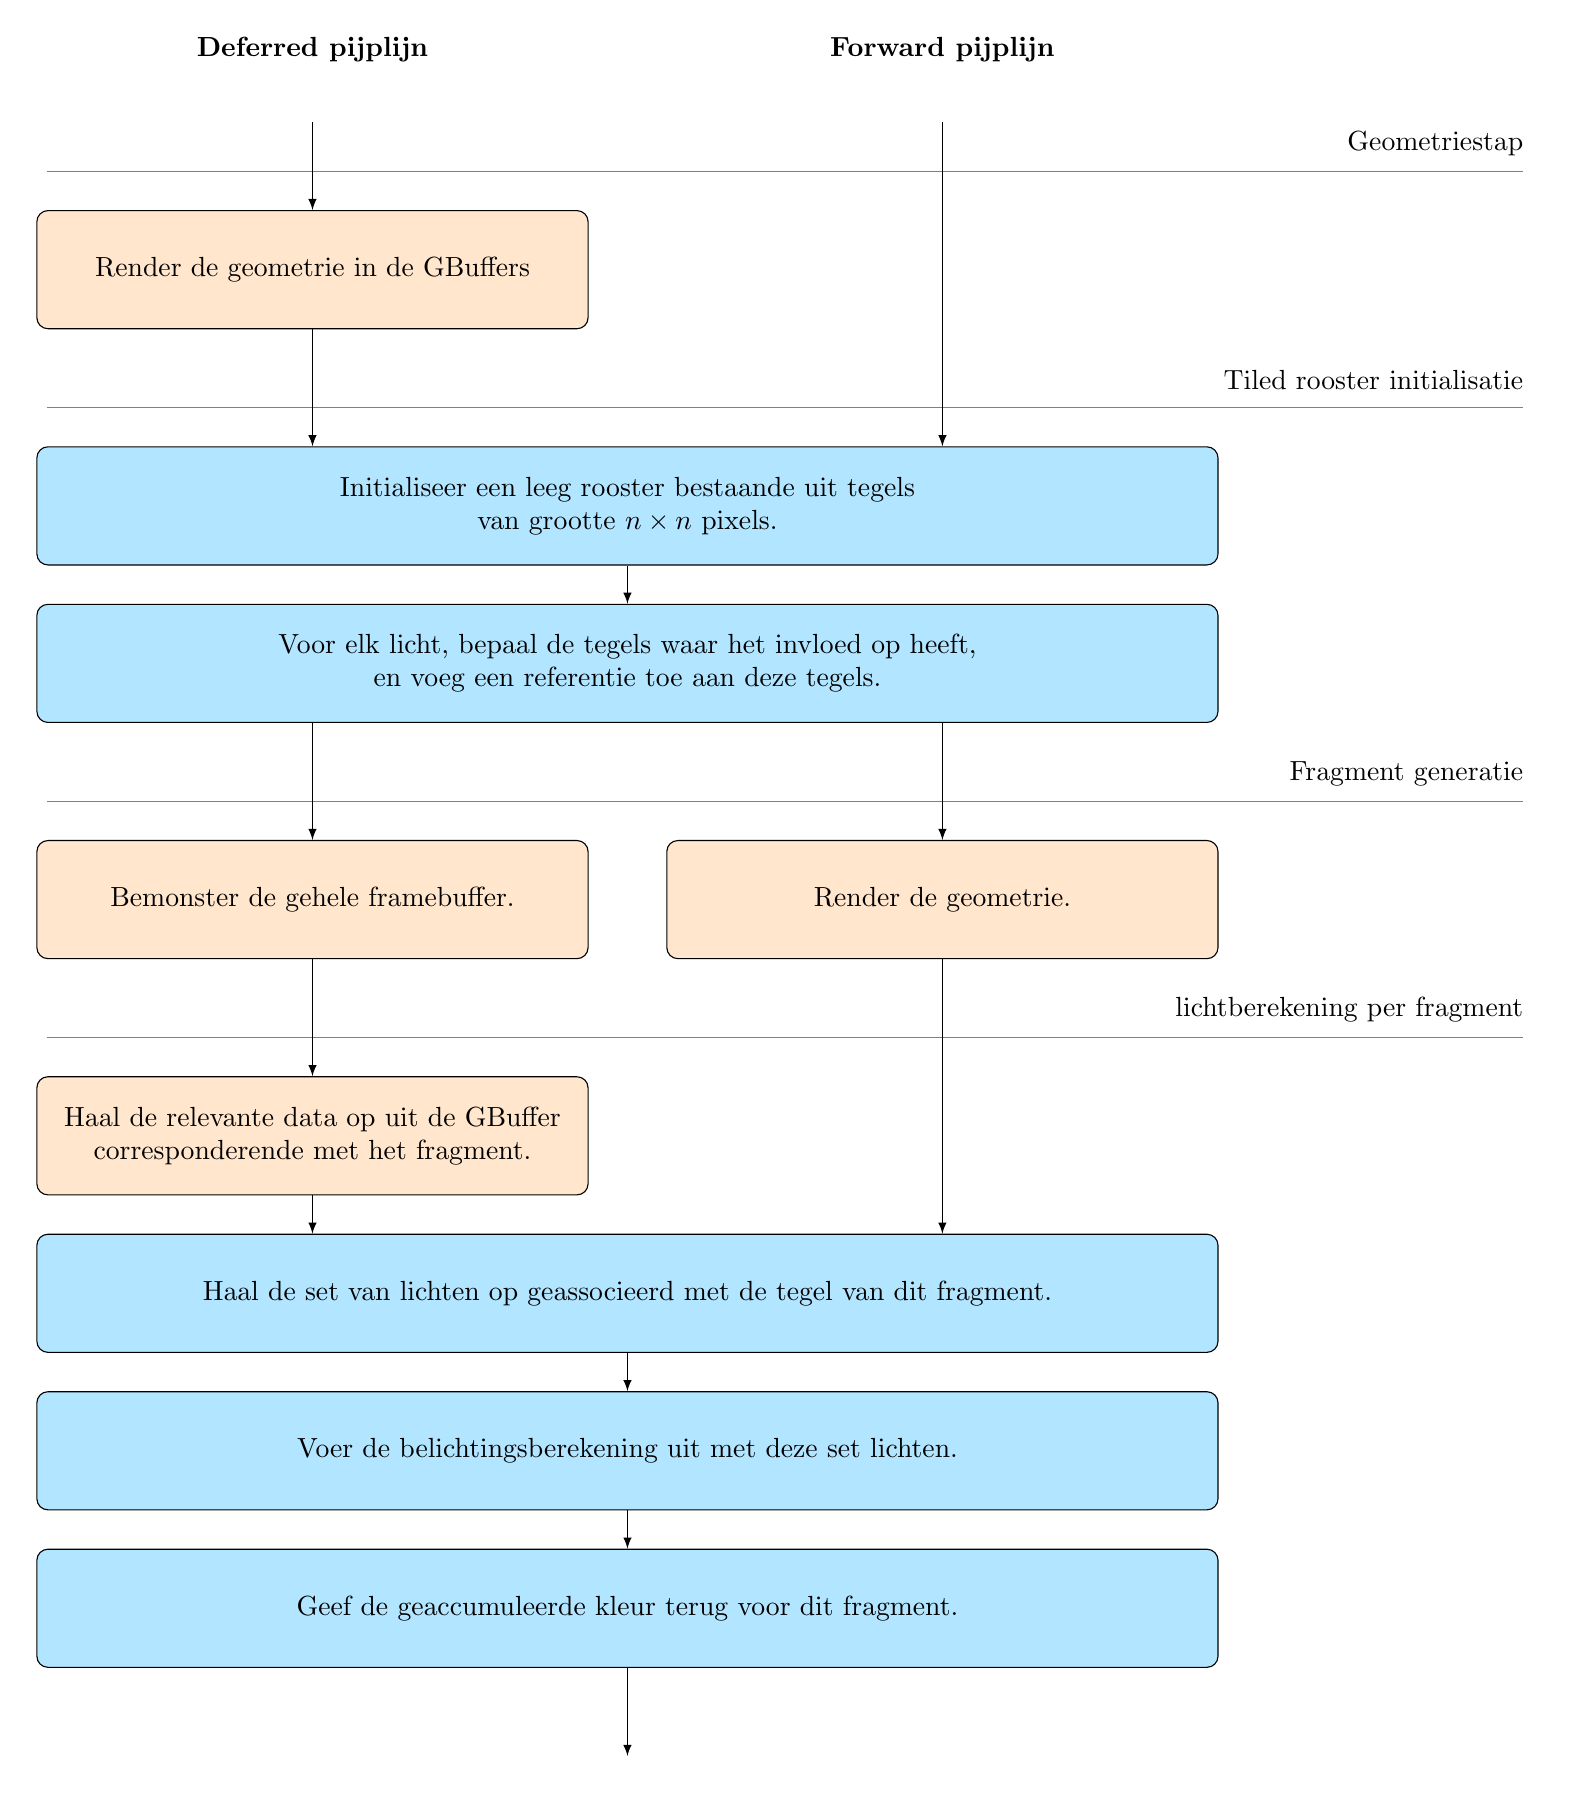
\begin{tikzpicture}[node distance=1.5cm
                      every node/.style={fill=white}, align=center]
    % Steps
    % --------------------------------------------------------------------------
    \node at (-4,  3.8) (deferred_text) [] {\textbf{Deferred pijplijn}};
    \node at ( 4,  3.8) (forward_tex)   [] {\textbf{Forward pijplijn}};
    
    \node at (-4,  3.0) (deferred_in)   [] {};
    \node at ( 4,  3.0) (forward_in)    [] {};
    
    \node at (-4,  1.0) (deferred_step0) [pipeline] {Render de geometrie in de GBuffers};
    
    \node at (-4,  -2) (anchor_deferred_step1) [ts-anchor] {};
    \node at ( 4,  -2) (anchor_forward_step1)  [ts-anchor] {};
  
    \node at (0.0, -2) (step1) [tiled] { Initialiseer een leeg rooster bestaande uit tegels \\
                                         van grootte  $n \times n$ pixels. };
    \node at (0.0, -4) (step2) [tiled] { Voor elk licht, bepaal de tegels waar het invloed op heeft, \\ 
                                         en voeg een referentie toe aan deze tegels.  };
   
    \node at (-4, -4) (anchor_deferred_step2) [ts-anchor] {};
    \node at ( 4, -4) (anchor_forward_step2)  [ts-anchor] {};

    \node at (-4,  -7) (deferred_step3) [pipeline] {Bemonster de gehele framebuffer.};
    \node at ( 4,  -7) (forward_step3)  [pipeline] {Render de geometrie.};
    
    \node at (-4, -10) (deferred_step4) [pipeline] {Haal de relevante data op uit de GBuffer\\
                                                          corresponderende met het fragment.};

    \node at (-4, -12) (anchor_deferred_step5) [ts-anchor] {};
    \node at ( 4, -12) (anchor_forward_step5)  [ts-anchor] {};

    \node at ( 0, -12) (step5) [tiled] { Haal de set van lichten op geassocieerd met de tegel van dit fragment.};
    \node at ( 0, -14) (step6) [tiled] { Voer de belichtingsberekening uit met deze set lichten.};
    \node at ( 0, -16) (step7) [tiled] { Geef de geaccumuleerde kleur terug voor dit fragment.};
    \node at ( 0, -18) (out) [] { };

    % Step lines
    % --------------------------------------------------------------------------
    \node at ( -7.5, 2.25) (line_1_l) [] {};
    \node at ( 11.5, 2.25) (line_1_r) [] {};
    \draw[gray] (line_1_l) -- (line_1_r);
    \node at ( 11.5, 2.60) (line_1_text) [anchor=east] {Geometriestap};

    \node at ( -7.5, -0.75) (line_2_l) [] {};
    \node at ( 11.5, -0.75) (line_2_r) [] {};
    \draw[gray] (line_2_l) -- (line_2_r);
    \node at ( 11.5, -0.40) (line_2_text) [anchor=east] {Tiled rooster initialisatie};
  
    \node at ( -7.5, -5.75) (line_3_l) [] {};
    \node at ( 11.5, -5.75) (line_3_r) [] {};
    \draw[gray] (line_3_l) -- (line_3_r);
    \node at ( 11.5, -5.40) (line_3_text) [anchor=east] {Fragment generatie};
  
    \node at ( -7.5, -8.75) (line_4_l) [] {};
    \node at ( 11.5, -8.75) (line_4_r) [] {};
    \draw[gray] (line_4_l) -- (line_4_r);
    \node at ( 11.5, -8.40) (line_4_text) [anchor=east] {lichtberekening per fragment};

    % Arrows
    % --------------------------------------------------------------------------
    \draw[-latex] (deferred_in)    -- (deferred_step0);
    \draw[-latex] (deferred_step0) -- (anchor_deferred_step1);
    \draw[-latex] (forward_in)     -- (anchor_forward_step1);
  
    \draw[-latex] (step1) -- (step2);
  
    \draw[-latex] (anchor_deferred_step2) -- (deferred_step3);
    \draw[-latex] (anchor_forward_step2)  -- (forward_step3);
  
    \draw[-latex] (deferred_step3) -- (deferred_step4);
    \draw[-latex] (deferred_step4) -- (anchor_deferred_step5);
    
    \draw[-latex] (forward_step3) -- (anchor_forward_step5);
  
    \draw[-latex] (step5) -- (step6);
    \draw[-latex] (step6) -- (step7);
    \draw[-latex] (step7) -- (out);
  \end{tikzpicture}
  \end{adjustbox}
  \caption{Het Tiled Shading algoritme voor de Forward en Deferred pijplijn.}
  \label{fig:ts-algorithm}
\end{figure}
